\chapter{Implementación}

Este capítulo tratará sobre las herramientas utilizadas para la implementación y planificación, así como los distintos algoritmos que se emplearán para realizar la simulación. Además, se detallará el diseño de los \textit{blueprints} y se describirán las reglas que seguirá el algoritmo de navegación.

\section{Herramientas utilizadas}

En el desarrollo del proyecto se utilizará \verb|git| para el control de versiones del proyecto y se almacenará en un repositorio de GitHub. 

\bigskip

Para el modelado y texturizado de los distintos objetos de la aplicación se utilizará Blender\cite{blender}. Asimismo, para la creación y modificación de las texturas se utilizará GIMP\cite{gimp}.

\bigskip

% En cuanto a herramientas para la planificación, se hará uso de la herramienta \planApp para llevar un control de las Historias de Usuario que se realizan y pendientes en cada Sprint.
En lo que respecta a herramientas de planificación, se utilizará \planApp para llevar un control de las historias de usuario realizadas y pendientes en cada sprint.

% foto de \planApp
\begin{figure}[H]
    \centering
    
\includegraphics[width=\textwidth]{imagenes/trello.png}
    \caption{Tablero de ejemplo de Trello\cite{tablero-trello}.}
\end{figure}

\section{Algoritmos utilizados}

Voy a dividir en subsecciones los diversos algoritmos que componen la simulación:

\subsection{Algoritmo para el giro del volante del coche}

En el control del volante de los vehículos, correspondiente a HU3 y realizada en el sprint 4, se ha utilizado un controlador PID (\textit{Proportional, Integral} y \textit{Derivative}). Este controlador se utiliza para regular el error de un sistema de manera suave y evitando producir muchas desviaciones mediante el ajuste de tres constantes para la componente proporcional, integral y derivativa. Cabe destacar que la variable a la que el sistema debe llegar se llama SP (\textit{Set Point}) y el valor actual del sistema se denomina PV (\textit{Process Variable}). 

% foto de una grafica de esas, quitar el bigskip si se encuentra alguna
% \caption{Diferencias de respuestas de un control estandar frente al controlador PID.}
\bigskip

Para que el controlador funcione bien, es necesario modificar sus tres constantes: 
% Proporcional, Integral y Derivativa. 

\begin{itemize}
    \item \textbf{Proporcional: }Actuará de manera proporcional al error actual, multiplicada por la constante asociada. Si solo se utiliza este componente, el sistema se pasará del SP, haciendo que tenga que volver a corregir, produciendo así demasiadas oscilaciones para llegar al SP. 

    \item \textbf{Integral: }Se encarga de derivar el error con respecto al tiempo, con el objetivo de anular errores residuales e incluso del propio sensor. Por normal general, seguirá pasándose del SP, ya que de esto se encarga la componente derivativa.

    \item \textbf{Derivativa: }Se utiliza para estimar como evolucionará la curva con el tiempo, basándose en su pendiente. Esta componente es la que se encarga de minimizar las oscilaciones, al reducir el efecto del actuador si se acerca demasiado rápido al SP.
\end{itemize}

\bigskip

% foto de la constante
\begin{figure}[H]
\centering
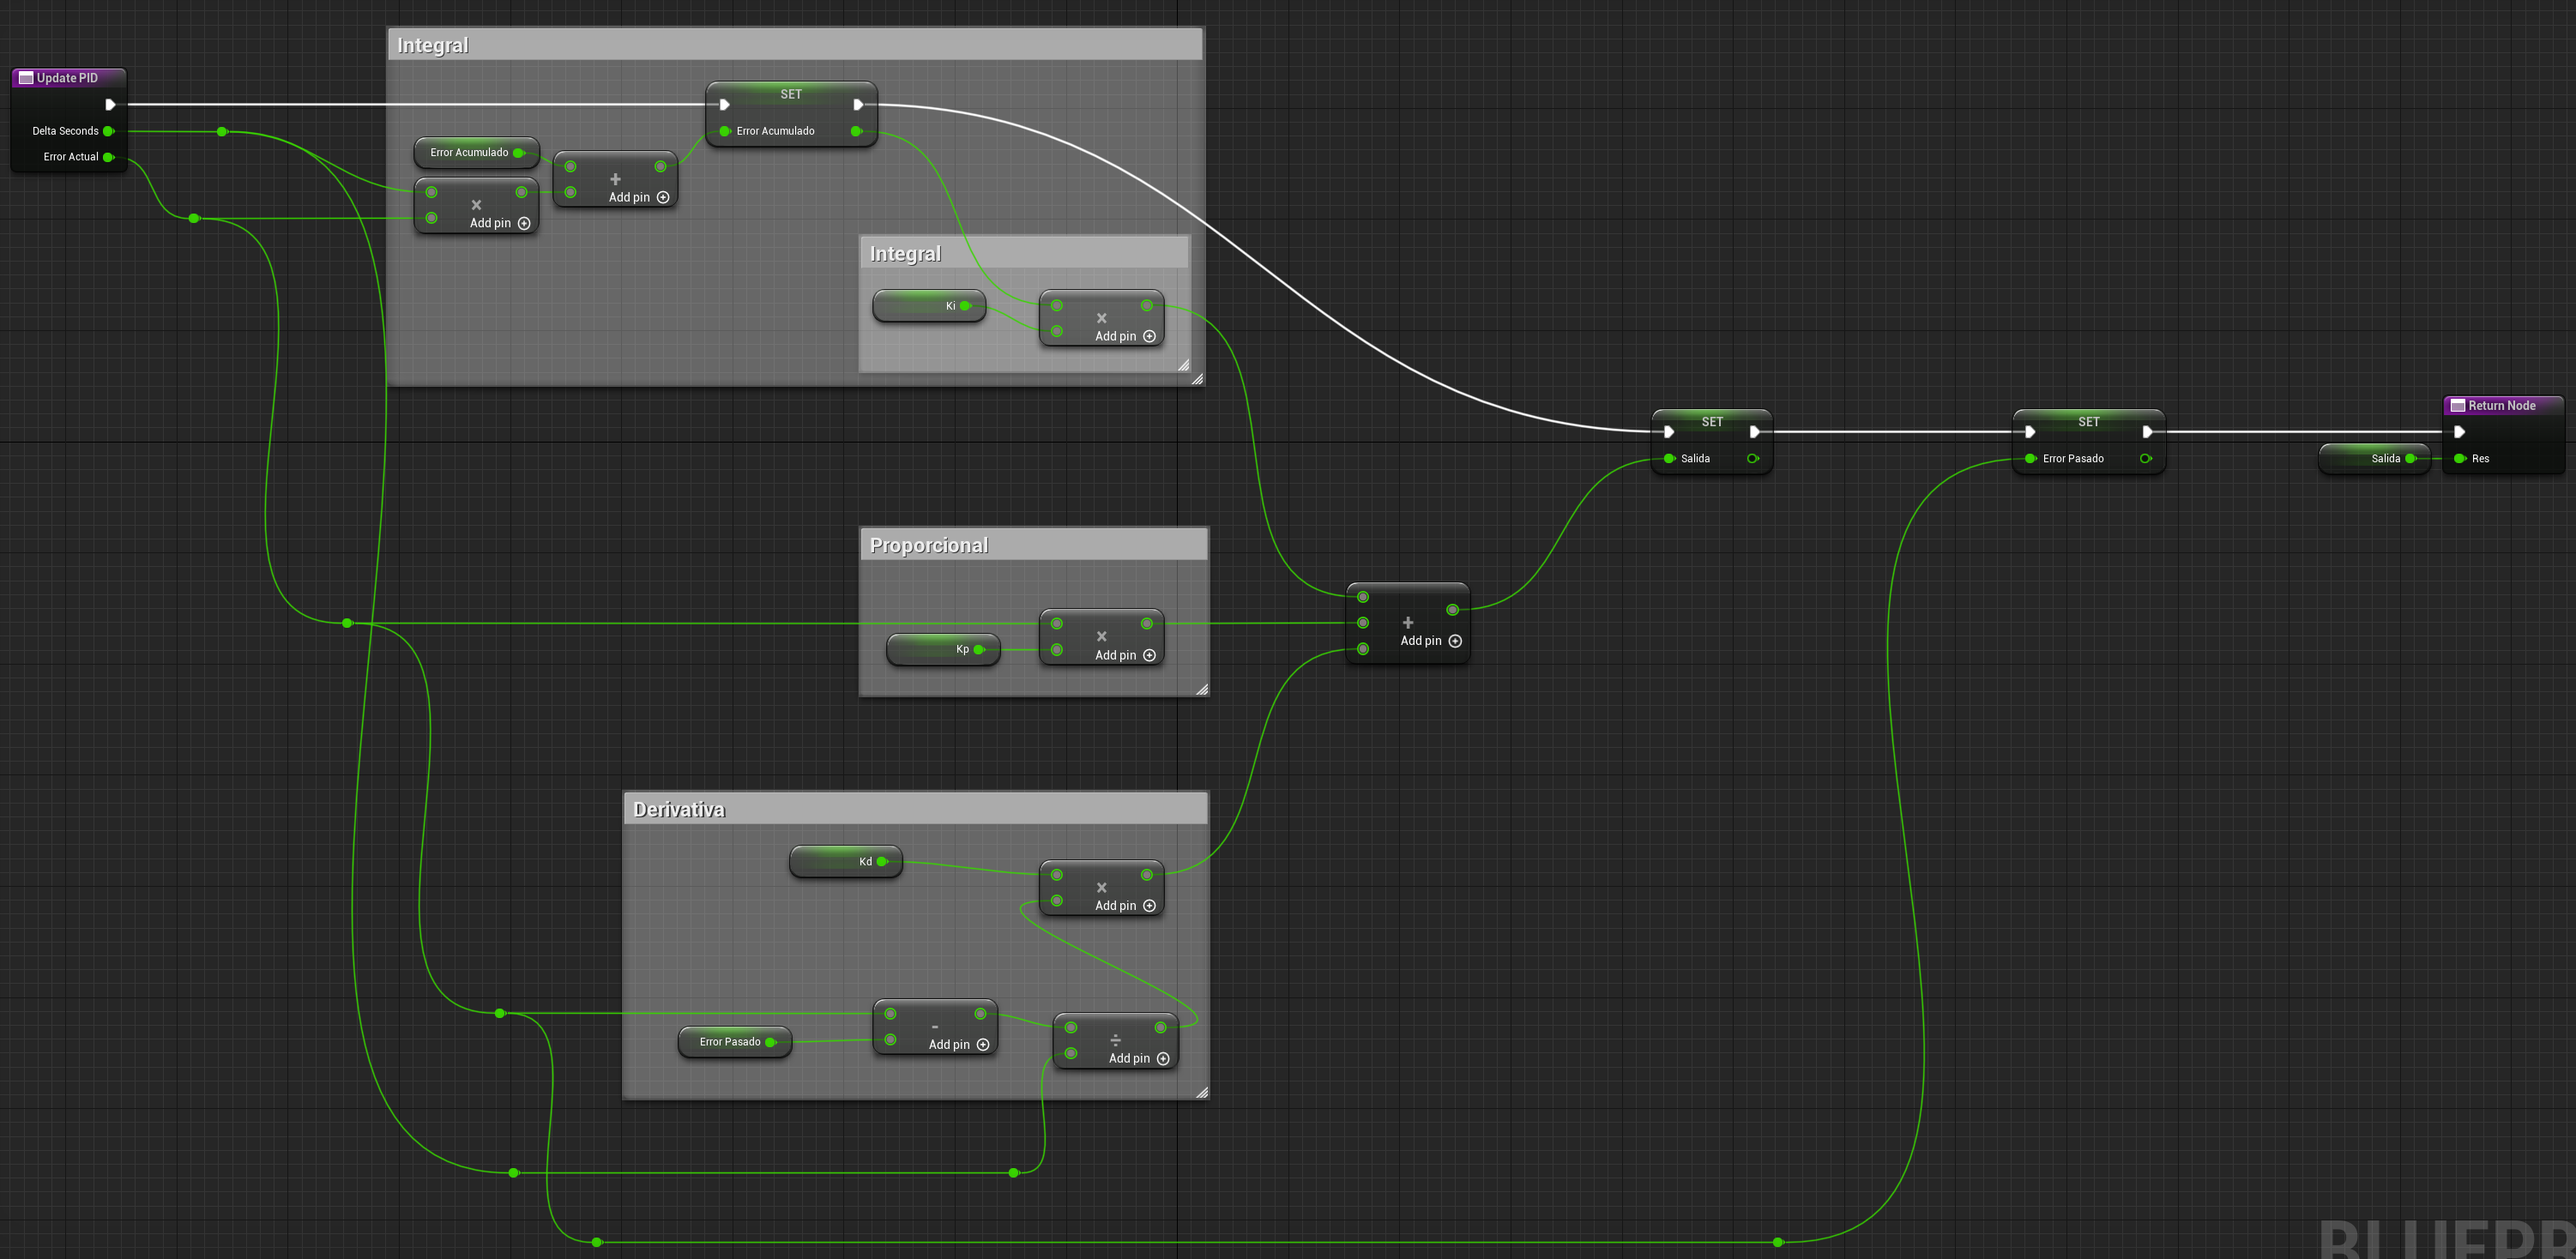
\includegraphics[width=\textwidth]{imagenes/PID-BP.png}
\caption{Implementación usando \textit{blueprints} del controlador PID.}
\end{figure}

El rango de valores que pueden tener las variables dependen del sistema al que se aplique. No obstante, todos los valores son números reales positivos, incluyendo el 0, que deshabilita la componente.

\bigskip

Cabe destacar que, en mi caso, el SP es el punto más cercano del coche a la ruta generada, y el error es la distancia del coche a dicho punto.

\bigskip

% rescribir la ultima parte ... y utilizando tambien el valor...
La calibración del PID se realiza modificando las constantes asociadas a cada componente. Existen diversos métodos como el de Ziegler-Nichols \cite{enwiki:1140258750}, que consiste en modificar solo la parte proporcional, dejando las demás a 0, hasta que el sistema comience a oscilar de manera estable, en ese momento se debe calcular la frecuencia a la que oscila y utilizando también el valor de la constante proporcional, se pueden obtener las demás mediante un cálculo matemático.

\bigskip

Dado que este método no me dio los resultados deseados, decidí implementar un algoritmo genético para obtener las constantes del controlador PID. Consiste en lanzar un conjunto de coches con valores de las constantes del PID aleatorios positivos al principio, con el objetivo de que intenten llegar a la meta con el menor error posible (por error se sigue entendiendo como la distancia del punto más cercano a la ruta con el coche). Aquellos con menos error, tienen más posibilidades de ser seleccionados para generaciones futuras. Una vez obtenido el error, se calcula su inversa y se obtiene la probabilidad de ser elegido mediante el nuevo valor entre la suma de todos. Esto dará como resultado unas probabilidades que al ser sumadas darán 1 (100\%). 

\bigskip

La selección se realiza lanzando una ruleta\cite{enwiki:1141636554}, cuyos sectores son divididos en función de la probabilidad calculada anteriormente. La ruleta se debe lanzar tantas veces como padres se desea tener. Una vez que se han elegido los coches que van a ser padres, se emparejan y se mezclan sus constantes para obtener dos hijos de cada pareja. Después, una de las tres constantes del PID en algunos de los hijos puede ser mutada, con una probabilidad del 33\%, con un valor aleatorio de rango [-0.1,0.1] que se le añade al valor existente. Finalmente se sustituyen los coches no elegidos para la siguiente generación por los hijos con las constantes mezcladas y mutadas, manteniendo a los padres, y se vuelve a ejecutar de nuevo el algoritmo.

\bigskip

Utilizando este algoritmo, obtuve unos valores que funcionaban bien para el circuito. No obstante, tras ejecutar varias veces el algoritmo, me he dado cuenta de que la constante integral siempre tiende a 0. Para solucionarlo, he decidido obligarle a que tenga un valor mínimo de 0,01.

% Queda por hablar de: adelantamientos, recuperacion despues de accidente, sistema de checkpoints, recuperacion de vuelco
\subsection{Algoritmos de navegación}

En cuanto al algoritmo de navegación, correspondiente a HU2, HU4 y HU5 e implementadas en los sprints 5 y 6, he utilizado A*\cite{enwiki:1152315016}, que es lanzado utilizando diversas reglas, y una componente reactiva. 

\bigskip

Para que el algoritmo A* pueda funcionar, es necesario discretizar el espacio de alguna forma, para que pueda ser ejecutado. Para ello, he decidido dividir el circuito en una malla de cubos de \cubeSize y con una cantidad de \gridSize cubos. Estos parámetros pueden ser modificados fácilmente, permitiendo albergar circuitos de mayor tamaño.

\bigskip

% Voy a dividir cada una de las partes que conforman el mapa en subsecciones:
En las siguientes subsecciones se explicará en detalle cada componente que forma la malla:

\subsubsection{Nodo}

Para implementarlo, he creado un actor que representa un nodo. Además, posee las variables necesarias para saber si se encuentra un vehículo dentro de él, si es un delimitador de límites de pista, si es un checkpoint o si es una guía de ruta óptima. De esta forma se puede tener un control muy alto sobre los pesos de cada estado.

\bigskip

La actualización de un nodo de un estado a otro se realiza mediante el evento \textit{ActorBeginOverlap} y \textit{ActorEndOverlap}. Así se puede actualizar el mapa en tiempo real.

\bigskip

Cabe destacar que los nodos con estado checkpoint y delimitador no pueden ser cambiados de estado; es decir, el delimitador de pista siempre estará ocupado, dándole un coste mayor. Mientras que el checkpoint siempre estará libre, dándole un coste menor. Los checkpoints nunca reciben colisión para optimizar la velocidad del algoritmo A*, ya que si se tienen en cuenta puede llegar a tardar demasiado en encontrar la ruta.

\bigskip

El estado ruta óptima sirve para darle una ayuda a los coches, ya que si no se utilizase escogería rutas más rígidas. Este estado no prohíbe a los coches la posibilidad de elegir otra ruta para adelantar o volver a pista, solo es una guía.

\bigskip

La construcción del delimitador y de la ruta óptima la he realizado utilizando actores distintos, de manera que se activen los eventos anteriormente mencionados para que se ajusten.

\bigskip

Por último, cada nodo también almacena una referencia a sus nodos adyacentes, para que puedan ser utilizados por el algoritmo A*.

\subsubsection{Malla de navegación}

Para realizar la malla de navegación he utilizado un actor encargado de generar los nodos mencionados anteriormente en una malla de \gridSize. Como he dicho antes, estos valores pueden ser modificados, incluido el offset de donde comienza a generar nodos.

\bigskip

Este actor incluye los métodos necesarios para poder direccionar un nodo de la malla como una matriz (con filas y columnas), poder obtener su posición en coordenadas del mundo y poder convertir de coordenadas del mundo a coordenadas de matriz.

\subsubsection{Algoritmo A*}

% rescribir
A* es utilizado para obtener rutas en un grafo. Para ello, hace uso de una función heurística para estimar la distancia restante al nodo destino. A diferencia de otros algoritmos, como el de Dijkstra, A* es más rápido, gracias a la heurística, ya que puede descartar nodos que están más alejados del destino.

\bigskip

El algoritmo se encarga de visitar todos los nodos vecinos, calculando el coste de llegar desde el origen y el coste para llegar al destino mediante la heurística, en caso de encontrar una ruta mejor de un nodo ya existente en la lista de abiertos, se elimina el anterior y se introduce el nuevo. Este proceso se repite hasta que se llega al destino o, en mi caso, llega a un límite de iteraciones.

\bigskip

Dado que la implementación convencional de A*, haciendo uso de una lista de abiertos para los nodos por visitar y otra de cerrados para los nodos ya visitados, me daba muchos problemas de rendimiento. He decidido mejorarlo eliminando la lista de cerrados y la comprobación de la existencia de una ruta mejor para un nodo que ya se encuentre en la lista de abiertos\cite{a-star}. Esta modificación tiene como desventaja que un mismo nodo puede estar varias veces en la lista de abiertos, pero suele dar mejores resultados\cite{Chen2007PriorityQA}.

\bigskip

Otra mejora ha sido la de utilizar una cola con prioridad para la lista de abiertos, de manera que siempre se encuentre al final (el primero para salir) aquel con menor coste.

\bigskip

Gracias a la cola con prioridad, la desventaja de la nueva versión de A* puede ser solucionada, al priorizarse la ruta más eficiente.


\subsubsection{Heurística}

Debido a que un nodo puede moverse en 8 direcciones distintas, incluyendo las diagonales, es necesario utilizar una heurística acorde. Por tanto, he decidido utilizar la distancia Chebyshev\cite{enwiki:1149051498}, cuyos movimientos diagonales tienen el mismo coste que los demás. 

\bigskip

La configuración de los nodos prohíbe utilizar una heurística como la distancia Manhattan, ya que sobrestimaría la distancia al destino, haciendo que no sea correcto.

\subsubsection{Cálculo de la ruta por los vehículos}

Con todo lo anterior implementado el coche es capaz de obtener una ruta por el circuito. No obstante, sigue siendo demasiado costoso obtener una ruta demasiado larga, para luego tener que desecharla por un adelantamiento o un choque. Es por eso que he dividido el circuito en varios checkpoints de tamaño relativamente reducido, con el objetivo de que el cálculo de rutas sea más rápido.

\bigskip

Cuando la parte delantera del vehículo se solapa con un checkpoint, calcula la ruta utilizando A* hasta el siguiente checkpoint. La llamada al algoritmo devuelve un vector de puntos en coordenadas del mundo. El vehículo se encarga de filtrar los puntos que quedan fuera del checkpoint solapado, con el objetivo de que resulte en una ruta más limpia. Para ello, calcula el producto escalar entre el \textit{Forward Vector} del checkpoint y el vector formado por el checkpoint y el cubo, si resulta que es menor o igual que 0 se elimina, ya que indica que se encuentra detrás.

\bigskip

Con los puntos filtrados, el coche construye un spline y pinta los puntos en el suelo. Este spline será seguido gracias al controlador PID mencionado anteriormente. Cabe destacar que al ser la ruta discreta y el vehículo una componente física del mundo, el vehículo no siempre conseguirá seguirla siempre, pero le servirá como ``guía'' a la hora de tener que hacer giros y adelantamientos.

\subsubsection{Lógica de adelantamiento de los vehículos}

Dado que el algoritmo A* funciona principalmente para mundos estáticos, es necesario actualizar la ruta si se realiza un cambio de posición en los vehículos. En este caso, para adelantar al contrincante.

\bigskip

La regla que sigue el vehículo es si se encuentra a una distancia del vehículo de adelante, ejecuta el algoritmo de navegación y espera unos pocos segundos para volverlo a ejecutar. Esta implementación me ha dado unos resultados razonables en tiempo y habilidad en los pilotos.

\subsubsection{Recuperación después de un accidente}

Si un coche se sale de pista primero se esperan unos segundos para comprobar que de verdad no se puede mover. Cuando se ha comprobado, se recorre un cierto tiempo marcha atrás con las ruedas rectas. Finalmente, ejecuta el A* para calcular una ruta de escapatoria y recorre lento dicha ruta por un breve instante de tiempo, hasta que finalmente recupera la velocidad que tenía.

\subsubsection{Recuperación después del vuelco}

Puede darse el remoto caso de que un vehículo vuelque y no sea capaz de darse la vuelta. En este caso he decidido implementar una regla que comprueba si la rotación del coche es mayor de 90 grados en ambos sentidos, pone el coche de nuevo sobre sus cuatro ruedas.

\subsection{Control de acelerador y freno}

El control del acelerador y del freno en condiciones normales de carrera se implementa incluyendo en cada checkpoint la velocidad recomendada a la que debe ir el coche. El coche calcula la distancia a la que se encuentra del siguiente checkpoint y la distancia de frenado necesaria basándose en la velocidad y la desaceleración por el frenado (también se incluye la componente de agresividad, que se explicará más tarde).

\bigskip

Cabe destacar que esta velocidad es modificada por el estado del piloto, que se explicará en secciones posteriores.

\subsection{Algoritmo para las posiciones de los pilotos}

En lo que se refiere al cálculo de las posiciones de cada piloto, correspondientes a HU7 y HU8 e implementadas en el sprint 7, he utilizado una estructura de datos algo más compleja. Los vehículos almacenan la vuelta en la que están y el checkpoint; es decir, el sector del circuito en el que se encuentran. Con la información anterior, he creado un array asociativo que almacene como clave la vuelta y como valor otro array asociativo, que a su vez tiene como clave el checkpoint y como valor un array con todos los vehículos que se encuentran en ese estado. Para mostrarlo, solo hace falta iterar primero por aquellas claves mayores, ya que son los que más vueltas y más lejos del circuito están.

% foto de la estructura de datos
% \usepackage{multirow}

\begin{table}[H]
    \centering
    \begin{tblr}{
        cells = {c},
        row{1} = {Silver},
        cell{1}{2} = {c=2}{},
        cell{2}{1} = {r=4}{},
        cell{2}{2} = {Alto},
        cell{2}{3} = {Alto},
        cell{7}{1} = {r=2}{},
        cell{7}{2} = {Alto},
        cell{7}{3} = {Alto},
        vlines,
        hline{1-2,6-7,9} = {-}{},
        hline{3-5,8} = {2-3}{},
            }
        \textbf{Clave (vuelta actual)} & \textbf{Valor }                    &                \\
        0                              & \textbf{Clave (checkpoint actual)} & \textbf{Valor} \\
                                       & 0                                  & {[}c1]         \\
                                       & ...                                &                \\
                                       & i                                  & {[}c2, c3]     \\
        ...                            & ...                                & ...            \\
        i                              & \textbf{Clave (checkpoint actual)} & \textbf{Valor} \\
                                       & 3                                  & {[}c4]
    \end{tblr}
    \caption{Representación de la estructura de datos que almacena las posiciones de los pilotos durante la carrera.}
\end{table}

% Para saber cuando lanzar la actualización de la lista de posiciones, cada coche calcula si el que está por delante de él sigue así, en caso contrario lanza el evento de actualización.

Para saber cuando lanzar la actualización de la lista de posiciones, cada coche comprueba si ha conseguido adelantar al coche que estaba inmediatamente delante de él, en caso afirmativo lanza el evento de actualización.


\subsection{Contador de vueltas}

En cuanto a la actualización del contador de vueltas, correspondiente a HU9 y realizado en el sprint 8, he hecho que todos los coches cuando acaben una vuelta intenten actualizarlo, en caso de que la vuelta actual sea mayor o igual, no se actualiza. De esta forma, es más fácil llevar un control más preciso de las vueltas.

% ver si es a partir del tercer piloto la agresividad
\subsection{Estado de los pilotos}

El estado de los pilotos está compuesto por tres parámetros: experiencia, agresividad y estado físico y mental.

\bigskip

La experiencia determina la rapidez con la que un piloto se pone agresivo, de forma que si es más experimentado, tardará más en llegar al máximo de agresividad. También permitirá que tenga algo más de aguante físico, al tener más experiencia.

\bigskip

El aguante físico y mental va bajando a lo largo de la carrera de manera periódica. Sus efectos se traducen en una pérdida de velocidad punta.

\bigskip

Mientras que la agresividad aumenta a partir del tercer piloto (inclusive) y disminuye cuando se encuentra entre los dos primeros. La agresividad aumentará más rápido si el piloto se encuentra en posiciones peores del ranking. Sus efectos se traducen en una ganancia ligera de velocidad y frenadas tardías en las curvas.